\newpage
\subsection{Caso d'uso UC16: Login con Google+}
\label{UC16}
\begin{figure}[ht]
	\centering
	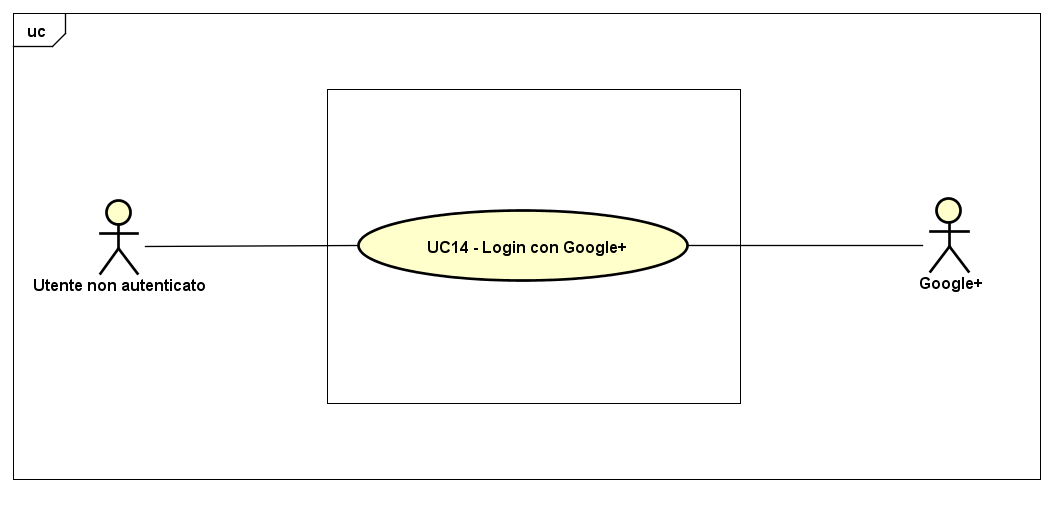
\includegraphics[scale=0.48]{UML/UC16.png}
	\caption{UC16: Login da Google+}
\end{figure}
\FloatBarrier
\begin{itemize}
	\item \textbf{Attori}: utente non autenticato, Google+;
	\item \textbf{Descrizione}: l'attore può autenticarsi utilizzando Google+;
	\item \textbf{Precondizione}: l'attore visualizza la pagina di login e sceglie il login con Google+;
	\item \textbf{Postcondizione}: l'attore è autenticato;
	\item \textbf{Scenario principale}: l'attore effettua il login tramite Google+.
\end{itemize}
